\documentclass[12pt]{article}
\usepackage{packages}
\usepackage[compat=1.1.0]{tikz-feynman}
\usepackage{verbatim}

\usepackage{biblatex}
\addbibresource{resources.bib}

\renewcommand*{\thesubsection}{}

% !TeX program = lualatex

\begin{document}

\thispagestyle{empty}

\centerline{\Large\bfseries Building supersymmetric models using superfields}
\vspace{10pt}
\centerline{\large Seminar on Supersymmetry and its breaking}
\vspace{10pt}
\centerline{Coordinated by prof. Joerg Jaeckel}

\vspace{30pt}

\begin{figure}[h]
  \centering
  
\includegraphics[scale=0.3]{images/uniheilogo.png}
\end{figure}
\vspace{30pt}


\centerline{\Large Matteo Zortea}
\vspace{10pt}
\centerline{University of Heidelberg, Department of Physics}
\vspace{10pt}
\centerline{Summer Semester 2022}


\vspace{50pt}
{
  \hypersetup{linkcolor=black}
  \tableofcontents
}

\newpage

\section{Introduction}
This paper is the write-up of a presentation in the seminar on Supersymmetry given at the University of Heidelberg in the Summer Semester 2022. In the previous presentations supersymmetry was introduced as an extension of the Poincarè group. Then the superspace and superfield formalism was presented and the formal properties were discussed. \par
\vspace{5pt}
\raggedright The main purpose of this paper is to show how this formalism naturally simplifies, at least conceptually, the description of supersymmetric theories. \\
After recalling some general properties of superfields, a general procedure to construct supersymmetric invariant lagrangians is presented. The simplest supersymmetric lagrangian that one can obtain is the free Wess-Zumino model; interactions are then added and the model is studied in a general way. 
Then some results on renormalization in SUSY are presented, namely the cancellation of the quadratic divergence in the scalar mass 1-loop correction and the N=1 nonrenormalization theorem. Gauge theories are then introduced first focusing on abelian groups, then moving on to general gauge groups. Finally interactions in SUSY QCD are studied qualitatively to look at peculiarities introduced by supersymmetry.
\subsection{How to build a SUSY lagrangian}
The first goal is to build a lagrangian $\mathcal{L}$ demanding that it transforms as
\begin{equation*}
  \mathcal{L} \to \mathcal{L} + \partial_\mu f(x)
\end{equation*}
under a supersymmetry transformation. This guarantees the theory to be supersymmetric invariant.
To do this let us move into a superspace with coordinates $\{x^\mu, \theta, \bar\theta\}$. The two main ingredients of a supersymmetric theory in the superspace formalism are the \emph{chiral} and \emph{vector superfields}. Let us briefly recall some of their properties, useful for the subsequent reasonings. \\
In superspace one defines two covariant derivatives
\begin{equation*}
  D_{\alpha} = \frac{\partial}{\partial \theta^\alpha} - i \sigma^\mu_{\alpha \dot\alpha} \overline{\theta}^{\dot\alpha} \partial_\mu \qquad\qquad \overline{D}^{\dot\alpha} = \frac{\partial}{\partial \overline{\theta}_{\dot\alpha}} - i \sigma^{\mu \alpha \dot\alpha}\theta_\alpha \partial_\mu
\end{equation*}
A \emph{left-chiral superfield} $\Phi$ (\emph{right-chiral superfield} $\chi$) is a superfield subject to the constraint $\bar D_{\dot \alpha} \Phi(x, \theta, \bar\theta) = 0$  ($D_{\alpha} \chi(x, \theta, \bar\theta) = 0$), and a general expansion in powers of $\theta, \bar\theta$ reads
\begin{equation}
\begin{gathered}
  \Phi(x, \theta, \bar\theta) = \varphi(x) + i\bar\theta \bar\sigma^{\mu}\theta \partial_{\mu}\varphi(x) + \frac{1}{4}\theta\theta\bar\theta\bar\theta\partial_{\mu}\partial^{\mu}\varphi(x) + \sqrt{2}\theta\psi(x) + \\ 
                -\frac{i}{\sqrt{2}}\theta\theta\bar\theta\bar\sigma^{\mu}\partial_{\mu}\psi(x) + \theta\theta F(x)
\end{gathered}
\label{eq:leftchiral_expansion}
\end{equation}
The hermitian conjugate of a left-chiral superfield $\Phi^*$ is a right-chiral superfield and vice-versa.
The field $\varphi$ entering equation \ref{eq:leftchiral_expansion} is the bosonic field of the theory, $\psi$ is its fermionic supersymmetric partner and $F$ will simply turn out to be unphysical. This will become clearer when looking at the interactions between the fields and at the equations of motion. \\
Under a SUSY transformation the components of a left-chiral superfield transform as 
\begin{gather*}
  \delta_{\epsilon} \varphi =\epsilon \psi \qquad\qquad
  \delta_{\epsilon} \psi_{\alpha} =-i\left(\sigma^{\mu} \epsilon^{\dagger}\right)_{\alpha} \partial_{\mu} \varphi+\epsilon_{\alpha} F, \qquad\qquad
  \delta_{\epsilon} F =-i \epsilon^{\dagger} \bar{\sigma}^{\mu} \partial_{\mu} \psi
\end{gather*}
The transformation law of $F$ is of particular interest, since it is precisely a total derivative, that is what one looks for to build invariant lagrangians. \par
\vspace{15pt}
\raggedright A vector superfield $V$ is obtained by imposing the reality condition $V=V^*$ on a general superfield, and an expansion in powers of $\theta, \bar\theta$ reads
\begin{gather*}
  V\left(x, \theta, \bar\theta\right) = a+\theta \xi+\bar\theta \xi^{\dagger} +\theta \theta b+\bar\theta \bar\theta b^*+\bar\theta \bar{\sigma}^{\mu} \theta A_{\mu}+ \\ 
                + \bar\theta \bar\theta \theta\left(\lambda-\frac{i}{2} \sigma^{\mu} \partial_{\mu} \xi^{\dagger}\right)
                +\theta \theta \bar\theta\left(\lambda^{\dagger}-\frac{i}{2} \sigma^{\mu} \partial_{\mu} \xi\right)+\theta \theta \bar\theta \bar\theta \left(\frac{1}{2} D+\frac{1}{4} \partial_{\mu} \partial^{\mu} a\right)
\end{gather*}
Here $A_\mu$ will be the spin-1 gauge field, with $\lambda$ beeing its fermionic supersymmetric partner. The field $D$ will drop out when looking at the equations of motion, while all the other degrees of freedom can be supergagued away by going in the Wess-Zumino gauge. \\
Under a SUSY transformation the components transform as 
\begin{gather*}
  \sqrt{2} \delta_{\epsilon} a =\epsilon \xi+\epsilon^{\dagger} \xi^{\dagger} \qquad 
  \sqrt{2} \delta_{\epsilon} \lambda_{\alpha} =\epsilon_{a} D+\frac{i}{2}\left(\sigma^{\mu} \sigma^{\nu} \epsilon\right)_{\alpha}\left(\partial_{\mu} A_{\nu}-\partial_{\nu} A_{\mu}\right) \\
  \sqrt{2} \delta_{\epsilon} b =\epsilon^{\dagger} \lambda^{\dagger}-i \epsilon^{\dagger} \sigma^{\mu} \partial_{\mu} \xi \qquad
  \sqrt{2} \delta_{\epsilon} \xi_{\alpha} =2 \epsilon_{\alpha} b-\left(\sigma^{\mu} \epsilon^{\dagger}\right)_{\alpha}\left(A_{\mu}+i \partial_{\mu} a\right) \\
  \sqrt{2} \delta_{\epsilon} A^{\mu} =i \epsilon \partial^{\mu} \xi-i \epsilon^{\dagger} \partial^{\mu} \xi^{\dagger}+\epsilon \sigma^{\mu} \lambda^{\dagger}-\epsilon^{\dagger} \bar{\sigma}^{\mu} \lambda \\
  \sqrt{2} \delta_{\epsilon} D =-i \epsilon \sigma^{\mu} \partial_{\mu} \lambda^{\dagger}-i \epsilon^{\dagger} \bar{\sigma}^{\mu} \partial_{\mu} \lambda
\end{gather*}
Here the term of interest is the field $D$ because it transforms precisely as a total derivative, as desired. Please note that even though they are called chiral and vector superfields, they don't carry any vector nor spinor indices; the name is only due to their particle content. \\
One now needs a way to select and isolate the desired components in order to keep only the invariant terms, that is $F$ for the chiral field and $D$ for the vector field. Integration of Grassman variables provides a natural way to accomplish this. Indeed 
\begin{equation}\begin{gathered}
  \int d^2\theta \, \Phi(x, \theta, \bar\theta) = \frac{1}{4} \, \bar\theta \bar\theta \partial_\mu \partial^\mu \varphi(x) - \frac{i}{\sqrt{2}} \bar\theta \bar\sigma^\mu \partial_\mu \psi(x) + F(x) = \\
  = F(x) + \text{total derivative} \equiv \left[\Phi\right]_F \\
  \int d^2\theta d^2\bar\theta \, V(x, \theta, \bar\theta) = \frac{1}{2} D + \frac{1}{4} \partial_\mu \partial^\mu a = \frac{1}{2} D + \text{total derivative} \equiv \left[V\right]_D
\end{gathered}
\label{eq:F_D_terms}
\end{equation}
The first meaningful supersymmetric lagrangian can be obtained by noting that the product $\Phi^*\Phi$ is real, hence a vector field. In particular, this implies that one can select the $D$ component $\left[\Phi^*\Phi\right]_D$ via integration to obtain a SUSY invariant lagrangian. \\
After writing the component-wise product $\Phi^*\Phi$, one can see that the D term (i.e. the coefficient of $\theta\theta\bar\theta\bar\theta$, compare with \ref{eq:F_D_terms}) results to be, after dropping total derivatives
\begin{gather*}
  \mathcal{L} = \int d^4 x \left[\Phi^*\Phi\right]_D = \int d^4 x \left( -\partial^\mu \varphi^* \partial_\mu \varphi + i \psi^\dagger \bar\sigma^\mu \partial_\mu \psi + F^*F \right)
\end{gather*}
This is the lagrangian of the \emph{Free Wess-Zumino model}. One can see that the kinetic term of the scalar field $\varphi$ comes with the kinetic term of the superpartner, the spinor $\psi$. The roles of $F, F^*$ will be understood later when looking at the equations of motion. \par 

\newpage 

\section{Wess-Zumino model}

We now want to proceed by adding interactions to the model. In order to do this one can observe that products of fields of the same chirality like $\Phi\Phi$, $\Phi^*\Phi^*$ are in turn chiral fields, since 
$\overline{D}_{\dot\alpha} \Phi\Phi = (\overline{D}_{\dot\alpha} \Phi) \, \Phi + \Phi (D_{\dot\alpha} \Phi) = 0$ ($D_\alpha \Phi^*\Phi^*=0$ follows analogously). More generally any holomorphic function of fields of the same chirality is in turn a chiral field with the same chirality, as it can easililly be seen by expanding it in power series. \\
Thus a function of the type
\begin{equation}
  W[\Phi] = a \, \Phi + \frac{1}{2!} \, m \, \Phi\Phi + \frac{1}{3!} \, y  \, \Phi \Phi \Phi
  \label{eq:superpotential}
\end{equation}
is certainly a left-chiral field, hence its $F$ component is SUSY invariant for what said in the previous section. We call $W[\Phi]$ the \emph{superpotential}. The lagrangian
\begin{gather*}
  \mathcal{L} = \left[\Phi^*\Phi\right]_D + \left[W[\Phi]\right]_F + \left[W^*[\Phi^*]\right]_F = \\
  = \int d^2\theta d^2\bar\theta \, \Phi^*\Phi + \int d^2\theta \, W[\Phi] + \int d^2 \bar\theta \, W^*[\Phi^*] 
\end{gather*}
is thus supersymmetric invariant. By using the property $\overline{DD}(\theta\theta) = -\frac{1}{4} = DD(\bar\theta\bar\theta)$ one can rewrite the D term as an F term and the lagrangian becomes
\begin{align*}
  \mathcal{L} &= \int d^2\theta \, \left(-\frac{1}{4} \, \overline{DD}(\Phi^*\Phi) + W[\Phi]\right) + \int d^2\bar\theta \, W^*[\Phi^*] \\
  &= \int d^2\theta \, W[\Phi] + \int d^2\bar\theta \left(-\frac{1}{4} \, DD(\Phi^*\Phi) + W^*[\Phi^*]\right)
\end{align*}
This allows one to derive the equations of motion for the superfields straightforwardly
\begin{equation*}
  \overline{DD} \Phi^* = 4\frac{\delta W}{\delta \Phi} \qquad\qquad  DD\Phi = 4\frac{\delta W^*}{\delta \Phi^*}
\end{equation*}
The superpotential in equation \ref{eq:superpotential} can be straightforwardly generalised to an arbitrary number of chiral superfields \
\begin{equation*}
  W[\Phi_i] = \sum_i a_i \, \Phi_i + \frac{1}{2!} \, m_{ij} \, \Phi_i\Phi_j + \frac{1}{3!} \, y_{ijk} \Phi_i \Phi_j \Phi_k
\end{equation*}
Note that in principle one is allowed keep higher orders in the power sum, but higher order terms would lead to a non renormalizable theory. To show this, let us do some dimensional analysis. \\
From the superfield expansion \ref{eq:leftchiral_expansion} one can note that the superfield and the bosonic field carry the same dimension $[\Phi] = [\varphi] = E^1$. If we want $\psi$ to be the fermionic 
superpartner of $\varphi$ then it must be a spinor with the usual dimension $[\psi] = E^{1/2} = [\psi^\dagger]$. This implies that it must be $[\theta] = E^{1/2} = [\bar\theta]$. \\ 
As known, the lagrangian must have dimension $E^4$, hence so  
it must be the dimension of $[W]_F = \int d^2\theta \, W[\Phi]$. Integrals in Grassman variables "act as derivatives", hence $[d^2\theta] = [d^2\bar\theta] = E^{-1}$, hence the dimension of the superpotential $W$ is $E^3$. \\
Finally, by looking at \ref{eq:superpotential}, one has that $[a] = E^2, [m] = E^1, [y] = E^0$, confirming that higher order terms would be non renormalizable. A similar reasoning forbids forbids also terms like $(\Phi^*\Phi)(\Phi^*\Phi)$ which would require a coupling constant with negative energy dimension.

\vspace{15pt}

Let us now write down the lagrangian in terms of components of the fields $\Phi, \Phi^*$
\begin{gather*}
  \mathcal{L} = \mathcal{L}_{WZ, D} + \mathcal{L}_{WZ, F} = \\ 
  = F^{*} F+\left(\partial_{\mu} \varphi\right)\left(\partial^{\mu} \varphi\right)^{*}+\frac{i}{2} \psi \sigma^{\mu}\left(\partial_{\mu} \psi^{\dagger}\right)-\frac{i}{2}\left(\partial_{\mu} \psi\right) \sigma^{\mu} \psi^{\dagger} + \\
      -m \varphi F-\frac{m}{2}(\psi \psi)-\frac{y}{2} \varphi \varphi F-\frac{y}{2} \varphi(\psi \psi)+\text { h.c. }
\end{gather*}
This allows one to derive the equations of motion for $F$ and $F^*$ straightforwardly 
\begin{gather*}
  F^{*} = m \varphi+\frac{y}{2} \varphi \varphi \qquad F = m\varphi^* + \frac{y}{2}\varphi^*\varphi^* 
\end{gather*}
These are algebraic equations which allow one to express directly $F, F^*$ as a function of $\varphi, \varphi^*$. By inserting the expressions in the lagrangian one gets 
\begin{equation}
  \begin{aligned}
      \mathcal{L}_{\mathrm{WZ}} &=\left(\partial_{\mu} \varphi\right)\left(\partial^{\mu} \varphi\right)^{*}+\frac{i}{2} \psi \sigma^{\mu}\left(\partial_{\mu} \psi^{\dagger}\right)-\frac{i}{2}\left(\partial_{\mu} \psi\right) \sigma^{\mu} \psi^{\dagger} \\
      &-|M|^{2} \varphi \varphi^{*}-\frac{|y|^{2}}{4} \varphi \varphi \varphi^{*} \varphi^{*}-\left(\frac{M}{2} \psi \psi+\frac{M \cdot y}{2} \varphi \varphi \varphi^{*}+\frac{y}{2} \varphi \psi \psi+\text { h.c. }\right)
      \end{aligned}
      \label{eq:lagrangian_components}
\end{equation}
This expression allows one to study the interactions and draw Feynman diagrams. Before doing so, let us give two comments 
\begin{itemize}
  \item In the last step the equations of motion were inserted in the lagrangian: this step should be taken with some care. In principle, the action can be evaluated for any configuration of the fields $\Phi(x, \theta, \bar\theta), \Phi^*(x,\theta, \bar\theta)$, with values of $F, F^*$ that can be completely unrelated to the values of $\varphi, \varphi^*$. 
  When we look at the (classical) equations of motion $\delta S = 0$ we are constraining the action to be a local extremum. Thus the lagrangian \ref{eq:lagrangian_components} is not a general one but rather one that extremizes the action, which would correspond to physical processes in the classical framework. One typically says that it is the "on shell" expression.
  \item The lagrangian \ref{eq:lagrangian_components} can also be written in terms of a potential function of the bosonic fields $\varphi, \varphi^*$ only
  \begin{equation*}
    V(\varphi) \equiv W(\varphi) = a \, \varphi + m \, \varphi^2 + y \, \varphi^3
  \end{equation*}
  namely the superpotential \ref{eq:superpotential} evaluated at the bosonic field $\varphi$. With this definition one can easilly check that
  \begin{equation*}
    F = -\left|\frac{\partial V}{\partial \varphi}\right|^2
  \end{equation*}
  and 
  \begin{equation*}
    \begin{aligned}
        \mathcal{L}_{\mathrm{WZ}} &=\left(\partial_{\mu} \varphi\right)\left(\partial^{\mu} \varphi\right)^{*}+\frac{i}{2} \psi \sigma^{\mu}\left(\partial_{\mu} \psi^{\dagger}\right)-\frac{i}{2}\left(\partial_{\mu} \psi\right) \sigma^{\mu} \psi^{\dagger} \\
        &-\left|\frac{\partial V\left(\varphi\right)}{\partial \varphi}\right|^{2}-\frac{1}{2}\left(\frac{\partial^{2} V\left(\varphi\right)}{\partial \varphi \partial \varphi}\right) \psi \psi-\frac{1}{2}\left(\frac{\partial^{2} V\left(\varphi^*\right)}{\partial \varphi^{*} \partial \varphi^{*}}\right) \psi^{\dagger} \psi^{\dagger}
    \end{aligned}
\end{equation*}
\end{itemize}
The interactions predicted by the lagrangian \ref{eq:lagrangian_components} are resumed in the diagrams in figure \ref{fig:WZ_interactions}. Note a peculiar aspect which is also visible by inspecting the lagrangian \ref{eq:lagrangian_components}: one has a coupling between $\psi$ and $\psi$ or between $\psi^\dagger$ and  $\psi^\dagger$ but not between $\psi$ and $\psi^\dagger$: for example the mass term we would 
find in the Dirac lagrangian is here not present. The reason of this lies in the restriction of the superpotentials $W(\Phi), W^*(\Phi^*)$ as analytic functions of fields of one chirality, in the sense that, by expanding them in power series, one gets only interactions between fields of the same chirality. Interactions between fields with different chiralities will be introduced afterwards when studying gauge theories.
\begin{figure}[h]
  \centering 
  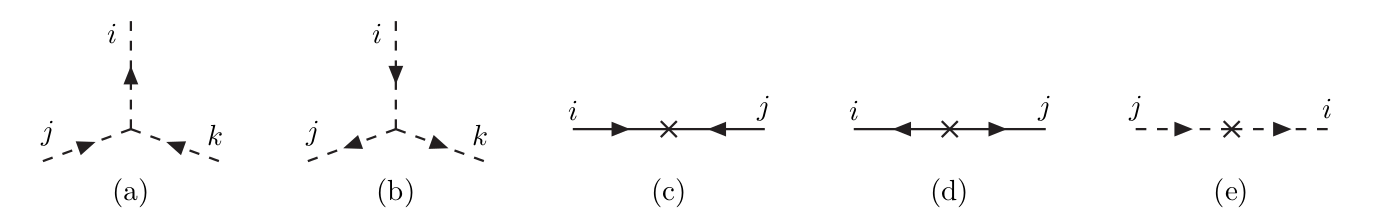
\includegraphics[scale=0.3]{images/feynman1.png}
  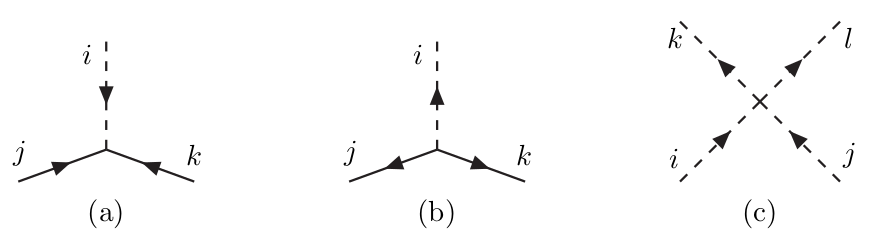
\includegraphics[scale=0.3]{images/feynman2.png}
  \caption{Interactions in the Wess-Zumino model given by the lagrangian \ref{eq:lagrangian_components}. The dashed lines represent the scalar component of the theory, while the continuous lines represent the fermionic superpartner. The diagrams are taken from ref. \cite{Signer_2009}.}
  \label{fig:WZ_interactions}
\end{figure}
\par 

\newpage

\section{Renormalization in N=1 supersymmetry}

\begin{figure}[h]
  \centering
  \feynmandiagram [scale=2., layered layout, horizontal=a to c, inline=(a.base)] {
  a -- [scalar, momentum={[arrow shorten=0.3]\(p\)}] b [dot],
  b -- [scalar, momentum={[arrow shorten=0.3]\(p\)}] c,
  b -- [out=135, in=45, loop, min distance=2cm, scalar, momentum={[arrow shorten=0.3]\(q\)}] b,
}; 
\quad + \qquad
\feynmandiagram [scale=2., layered layout, horizontal=b to c, inline=(a.base)] {
  a -- [scalar, momentum={[arrow shorten=0.3]\(p\)}] b [dot],
  b -- [fermion, half left, looseness=1.5, edge label=\(q\)] c [dot],
  b -- [fermion, half right, looseness=1.5, edge label=\(p-q\)] c,
  c -- [scalar, momentum={[arrow shorten=0.3]\(p\)}] d,
};
\caption{1-loop corrections to the scalar propagator with the lagrangian give by equation \ref{eq:lagrangian_components}}
\label{fig:scalar_mass_renormalization}
\end{figure}

In supersymmetry one often deals with precise cancellations of some diagrams due to the boson-fermion symmetry. As an example let us look at the scalar field's mass correction at one loop order. The two contributing diagrams are reported in figure \ref{fig:scalar_mass_renormalization}.
\raggedright The contribution from the first diagram is
\begin{gather*}
  I_1(p) = 4 \,\frac{i|y|^2}{4} \, \int \frac{d^4 q}{(2\pi)^4} \, \frac{i}{q^2 - m^2} = - |y|^2 \, \int \frac{d^4 q}{(2\pi)^4} \, \frac{1}{q^2 - m^2}
\end{gather*}
The contribution from the second diagram is 
\begin{gather*}
  I_2(p) = - 2 \, \left(\frac{iy}{2}\right)\left(\frac{iy^*}{2}\right) \int \frac{d^4 q}{(2\pi)^4} \, \text{Tr}\left[\frac{i(\sigma \cdot q + m)}{q^2 - m^2} \, \frac{i(\bar\sigma \cdot (p-q) + m)}{(p-q)^2 - m^2}\right] = \\
  - |y|^2 \, \int \frac{d^4 q}{(2\pi)^4} \, \frac{q\cdot p - q^2 - 2m^2}{(q^2-m^2) ((q-p)^2-m^2)}
\end{gather*}
where the property $\text{Tr}[\sigma_\mu \bar\sigma_\nu] = 2\eta_{\mu\nu}$ has been used. In order to calculate the mass correction, we have to evaluate the two expressions for $p=0$. Hence
\begin{gather*}
  I_1(0) + I_2(0) = -|y|^2 \int \frac{d^4q}{(2\pi)^4} \, \frac{1}{q^2-m^2} - \frac{q^2 -m^2 + m^2 + 2m^2}{(q^2-m^2)^2} \\
  -|y|^2 \int \frac{d^4q}{(2\pi)^4} \, \cancel{\frac{1}{q^2-m^2}} - \cancel{\frac{1}{q^2-m^2}} - \frac{3m^2}{(q^2-m^2)^2}= \\ 
  = 3m^2|y|^2 \int \frac{d^4q}{(2\pi)^4} \, \frac{1}{(q^2-m^2)^2}
\end{gather*}
The quadratically divergent term got cancelled in the second line and the result is now logarithmically divergent. \par 
\vspace{15pt}
A remarkable result which is here stated without proof \footnote{The proof can be found in ref. \cite{weinberg_1996}} is the so called \emph{N=1 nonrenormalization theorem}:
\begin{center}
  The superpotential is never renormalised at any order in perturbation theory. Thus it might be renormalised by non-perturbative effects such as istantons.
\end{center}

\newpage 

\section{Supersymmetric gauge theories}

\subsection{Abelian gauge theories}

We now want to introduce gauge invariance in the theory. At first let us focus on the abelian U(1) group, which will then be generalised to an arbitrary gauge group. 
Let us consider the Wess-Zumino lagrangian for an arbitrary number of superfields
\begin{equation*}
  \mathcal{L} = \int d^2\theta d^2\bar\theta \, \sum_i \Phi_i^\dagger \Phi_i + \int d^2\theta \left( \sum_i a_i \, \Phi_i + \sum_{ij} m_{ij} \, \Phi_i\Phi_j + \sum_{ijk} y_{ijk} \, \Phi_i\Phi_j\Phi_k\right) + h.c.
\end{equation*}
Let us first consider 
a global symmetry
\begin{equation}
  \Phi_i \to e^{iq_i \Lambda_i}\Phi_i \qquad \qquad \Phi^*_i \to \Phi^*_i e^{-iq_i \Lambda_i}
  \label{eq:gaugetransf_phi}
\end{equation}
The kinetic term $\int d^2\theta d^2\bar\theta \sum_i \Phi_i^\dagger \Phi_i$ is always invariant but the potential term is not. In fact the linear term is obviously not invariant, hence must be dropped. 
Moreover, whenever $q_i + q_j \neq 0$ we must require $m_{ij} = 0$ and whenever $q_i + q_j + q_k \neq 0$ we must require $y_{ijk} = 0$. Note in particular that the condition on the mass term implies $q_i = 0$ or $m_{ii} = 0$. \\
We now promote the global symmetry to a local symmetry, hence $\Lambda \to \Lambda(x, \theta, \bar\theta)$. One can now note that the generator is not a normal function but rather a superfield. Note that it cannot be an arbitrary one. 
In fact gauge symmetries are transformations which do not change the physical state of the system, but rather  one can say that configurations that differ by a gauge transformation are physically equivalent. This in particular means that a chiral field must be mapped into fields of the same chirality. 
By looking at equation \ref{eq:gaugetransf_phi} one can immediately conclude that $\Lambda(x, \theta, \bar\theta)$ must be a left-chiral superfield, hence $\Lambda^\dagger(x, \theta, \bar\theta)$ is a right-chiral superfield. This brings a problem in the kinetic term because 
\begin{equation*}
\Phi^* \Phi \to \Phi^* \, e^{-iq\Lambda^\dagger(x,\theta,\bar\theta)} \, e^{iq\Lambda(x,\theta,\bar\theta)} \, \Phi \neq \Phi^* \Phi
\end{equation*}
since due to the different chirality $\Lambda^\dagger \neq \Lambda $ unless they are both constant, which is the case of global symmetry. \\
The problem is analogous to the one that one finds in the kinetic term in standard QFT when one tries to make a lagrangian gauge invariant, and it is solved by manually adding compensation terms. In the case of standard QFT one
promotes the derivatives to gauge covariant derivatives, here we proceed by adding a factor $e^V$ between the two superfields, making the kinetic term to be $\Phi^* e^V \Phi$ where $V=V(x,\theta,\bar\theta)$ is a vector field. To see why this fixes the problem recall that a gauge transformation for any vector superfield $V$ is
\begin{equation*}
  V \to V + iq\left(\Lambda^\dagger(x, \theta, \bar\theta) - \Lambda(x, \theta, \bar\theta)\right)
\end{equation*}
which is precisely what we need
\begin{equation*}
  \Phi^* e^V \Phi \to \Phi^* e^{-iq\Lambda^\dagger } e^{V + iq(\Lambda^\dagger - \Lambda)} e^{iq\Lambda} \Phi = \Phi^* e^V \Phi
\end{equation*}
We must now specify a kinetic term for the gauge superfield $V(x, \theta, \bar\theta)$. This is accomplished by defining two chiral fields 
\begin{equation*}
  \mathcal{W_\alpha} \equiv -\frac{1}{4}\overline{DD}D_\alpha V \qquad \overline{\mathcal{W}}_{\dot\alpha} \equiv -\frac{1}{4}DD \overline{D}_{\dot\alpha} V
\end{equation*}
and building the two quantities
\begin{equation*}
  \mathcal{W}_{\alpha} \mathcal{W}^{\alpha} \equiv \mathcal{W}\mathcal{W} \qquad\qquad \overline{\mathcal{W}}_{\dot\alpha} \overline{\mathcal{W}}^{\dot\alpha} \equiv \overline{\mathcal{W}\mathcal{W}}
\end{equation*}
Remembering that product of superfields of the same chirality are in turn superfields of the same chirality and that the F term of a chirall field is supersymmetric invariant, the kinetic term becomes 
\begin{equation*}
  \left[\mathcal{W}\mathcal{W}\right]_F + \left[\overline{\mathcal{W}\mathcal{W}}\right]_F
\end{equation*}
The quantity is supersymmetric invariant by construction. One can make two further checks to verify that this is indeed a good choice for the kinetic term. One is gauge invariance which is straightforwardly proven using the anticommutation relation properties of the covariant derivatives $\left\{\bar{D}_{\bar\beta}, D_{\alpha}\right\}= - 2 i \sigma_{\alpha \dot{\beta}}^{\mu} \partial_{\mu}$
\begin{equation*}
  \begin{aligned}
      \mathcal{W}_{\alpha} \quad\to\quad \mathcal{W_\alpha}' &= -\frac{1}{4} \overline{D D} D_{\alpha}\left[V+i\left(\Lambda^{\dagger}-\Lambda\right)\right] =\mathcal{W}_{\alpha}+\frac{i}{4} \overline{D D} D_{\alpha} \Lambda \\
      &=\mathcal{W}_{\alpha}-\frac{i}{4} \bar{D}^{\dot{\beta}}\left\{\bar{D}_{\dot{\beta}}, D_{\alpha}\right\} \Lambda 
      =\mathcal{W}_{\alpha}+\frac{1}{2} \sigma_{\alpha \dot{\beta}}^{\mu} \partial_{\mu} \bar{D}^{\dot{\beta}} \Lambda
      =\mathcal{W}_{\alpha}
  \end{aligned}
\end{equation*}
The second is to check whether it contains the spin-1 gauge boson kinetic term. This can be done by expressing $V(x, \theta, \bar\theta)$ in compontents in the Wess-Zumino gauge and after a quite tedious but straighforward calculation one can show that 
\begin{equation*}
  \frac{1}{4} \, \left[\mathcal{W}\mathcal{W}\right]_F + \frac{1}{4} \left[\overline{\mathcal{W}\mathcal{W}}\right]_F = -\frac{1}{4} F_{\mu\nu}F^{\mu\nu} + i \lambda^\dagger \bar\sigma^\mu \partial_\mu \lambda + \frac{1}{2} \, D^2
\end{equation*}
Note that together with the usual spin-1 gauge boson kinetic term one also gets a kinetic term for the spinor $\lambda$. This the fermionic superpartner of the gauge boson, the \emph{gaugino}. In the case of $U(1)$ symmetry the two superpartners are the \emph{photon} and the \emph{photino}.
The D term drops out when looking at the equation of motion similarly to F. In fact the equations of motion for D are very straighforward since D is contained only in the kinetic terms through V. Noting that $[\Phi^* e^V \Phi]_D = \Phi^* \Phi D$ one has the equations of motion 
\begin{equation*}
  0 = \frac{\delta \mathcal{L}}{ \delta D} = D + \Phi^* \Phi
\end{equation*}
In the end the U(1) gauge invariant supersymmetric lagrangian is 
\begin{equation*}
  \mathcal{L} = \frac{1}{4} \, \left[\mathcal{W}\mathcal{W}\right]_F + \frac{1}{4} \left[\overline{\mathcal{W}\mathcal{W}}\right]_F + \left[\Phi^* e^V \Phi\right]_D + [W(\Phi)]_F + [\overline{W} (\Phi^*)]_F
\end{equation*}
\par
\vspace{15pt}

\subsection{General gauge theories}
The generalization to non-abelian gauge groups is conceptually straightforward, even though calculations become more complicated. Let us consider a gauge group $\mathcal{G}$ and its Lie algebra $Lie(\mathcal{G})$ with generators $\left\{T^a\right\}$.
Any element $A_\mu$ in the algebra can be written, in a given representation, as $A_\mu = \sum_a A_\mu^a \, T^a$. The problem is that now the kinetic term in the lagrangian transforms as 
\begin{equation*}
  \Phi^* e^V \Phi \to \Phi^* e^{-iq\Lambda} e^{V + iq(\Lambda^\dagger - \Lambda)} e^{iq\Lambda}
\end{equation*}
which is not $\Phi^* e^V \Phi$ because now the exponents have to be combined in a non trivial way using the Baker-Campbell-Hausddorf formula. The problem can be fixed by redefining the transformation properties of the vector superfield as 
\begin{equation*}
  e^V \to e^{i\Lambda^\dagger} e^V e^{-i\Lambda}
\end{equation*}
which implies 
\begin{align*}
  V \rightarrow &V + i\left(\Lambda^{\dagger}-\Lambda\right)-\frac{i}{2}\left[V, \Lambda+\Lambda^{\dagger}\right] 
  + i \sum_{k=1}^{\infty} \frac{B_{2 k}}{(2 k) !}\left[V,\left[V, \ldots\left[V, \Lambda^{\dagger}-\Lambda\right] \ldots\right]\right] = \\
  = & V + i\left(\Lambda^{a *}-\Lambda^{a}\right)+g_{a} f^{a b c} V^{b}\left(\Lambda^{c *}+\Lambda^{c}\right) 
  -\frac{i}{3} g_{a}^{2} f^{a b c} f^{c d b} V^{b} V^{d}\left(\Lambda^{c}-\Lambda^{r}\right)+\ldots
\end{align*}
where $B_n$ defined by $\frac{x}{e^{x}-1}=\sum_{n=0}^{\infty} \frac{B_{n}}{n !} x^{n}$ are the Bernoulli numbers. Note that this definition trivially reduces to the old one in the abelian case ($f^{abc}=0$). \\
The kinetic term of the gauge fields must also be redefined to take account of the new transformation law of $V$ and we write it as 
\begin{equation*}
  \mathcal{W}_\alpha = -\frac{1}{4} \overline{DD} (e^{-V}D_{\alpha}e^V)
\end{equation*}
As an example let us write down the lagrangian in components for supersymmetric QCD and let us study it qualitatively
\begin{equation}
  \begin{aligned}
      \mathcal{L} &=\left(D_{\mu} \varphi_{i}\right)^{*}\left(D^{\mu} \varphi\right)_{i}+\frac{i}{2} \psi_{i} \sigma^{\mu}\left(D_{\mu} \psi^{\dagger}\right)_{i}-\frac{i}{2}\left(D_{\mu} \psi\right)_{i} \sigma^{\mu} \psi^{\dagger}_{i}\\
      &-\frac{1}{4} F_{\mu \nu}^{a}\left(F^{a}\right)^{\mu \nu}+\frac{i}{2} \lambda^{a} \sigma^{\mu}\left(D_{\mu} \bar{\lambda}\right)^{a}-\frac{i}{2}\left(D_{\mu} \lambda\right)^{a} \sigma^{\mu} \bar{\lambda}^{a} \\
      &-\sqrt{2} i g \psi^{\dagger}_{i} \bar{\lambda}^{a} T_{i j}^{a} \varphi_{j}+\sqrt{2 i g} \varphi_{i}^{\dagger} T_{i j}^{a} \psi_{j} \lambda^{a} \\
      &-\frac{1}{2} \frac{\partial^{2} W}{\partial \varphi_{i} \partial \varphi_{j}} \psi_{i} \psi_{j}-\frac{1}{2} \frac{\partial^{2} W^{\dagger}}{\partial \varphi_{i}^{*} \partial \varphi_{j}^{*}} \psi^{\dagger}_{i} \psi^{\dagger}_{j}-V\left(\varphi_{i}, \varphi_{j}^{*}\right)
      \end{aligned}
  \label{eq:SQCD}
\end{equation}
where 
\begin{equation*}
    V\left(\varphi_{i}, \varphi_{j}^{*}\right)=F_{i}^{*} F_{i}+\frac{1}{2}\left(D^{a}\right)^{2}=\sum_{i}\left|\frac{\partial W}{\partial \varphi_{i}}\right|^{2}+\frac{1}{2} \sum_{a}\left(g \varphi_{i}^{*} T_{i j}^{a} \varphi_{j}+k^{a}\right)^{2}
\end{equation*}
\begin{equation*}
    W\left(\varphi_{i}\right)=a_{i} \varphi_{i}+\frac{1}{2} m_{i j} \varphi_{i} \varphi_{j}+\frac{1}{3 !} y_{i j k} \varphi_{i} \varphi_{j} \varphi_{k}
\end{equation*}
In the first line one can note the kinetic term for the quarks and the bosonic superpartners, the squarks. The covariant derivatives contain the terms which give the interaction between the gauge bosons and the chiral supermultiplet's fields. \\
In the second line there are the kinetic terms for the gluons and gluinos, together with their mutual interaction. In the third and fourth lines all the interactions with the gauginos. A peculiar and remarkable result is that the generators $T^a_{ij}$ play directly 
a role as coupling constants either for the chiral supermultiplet's fields to the gauginos (gluinos in this case) or between fermions with different chirality: remember that this interaction was not allowed in the Wess-Zumino model due to the assumption on the form of the superpotential (compare with the lagrangian \ref{eq:lagrangian_components} and figure \ref{fig:WZ_interactions}). \\
The resulting Feynman diagrams are reported in figure \ref{fig:SQCD_interactions}. \par
\vfill
\newpage

\begin{figure}[h]
  \centering 
  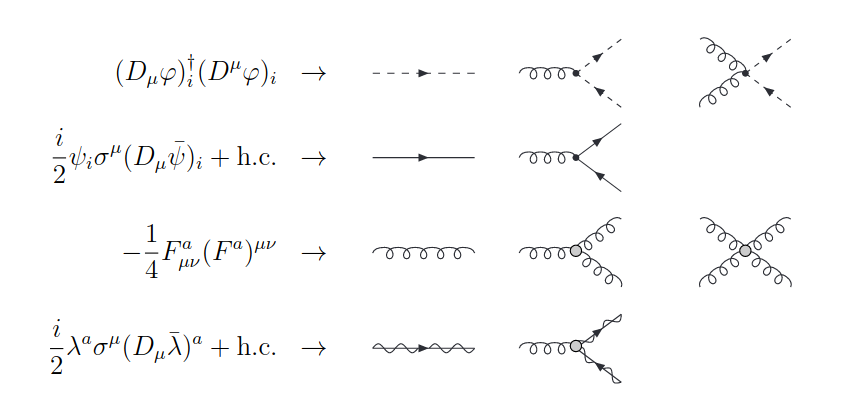
\includegraphics[scale=0.45]{sqcd_inter_2.png}
  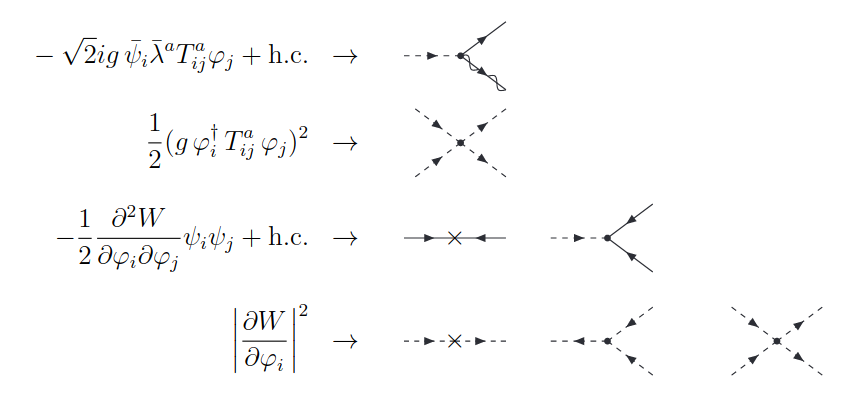
\includegraphics[scale=0.45]{sqcd_inter_1.png}
  \caption{Interactions in the supersymmetric QCD model given by the lagrangian \ref{eq:SQCD}. The diagrams are taken from ref. \cite{Signer_2009}}
  \label{fig:SQCD_interactions}
\end{figure}

\section{Conclusions and outlooks}
The main purpose of this paper was to show how the superspace formalism simplifies, at least conceptually, the description of supersymmetric theories. This was made clear in the derivation 
of the Wess-Zumino model, which was shown to be the simplest model that one can derive using only chiral superfields. The model was then generalised to gauge theories and SQCD was taken as an example. \\
\vspace{5pt}
One of the most remarkable results obtained was the cancellation of the quadratic divergence in the scalar field's mass 1-loop correction, which has striking consequences for the Higgs boson and the Standard Model in general.  
Thus, this happens precisely because superpartners enter in the theory with the same mass. This obviously cannot be correct, as for example we do not observe (yet) squarks and sleptons in experiments. This observation 
is one of the main motivations to then break supersymmetry, and the challenge will be to do so by mantaining the main features which motivated the introduction of the theory. These topics are discussed in the subsequent presentations.

\newpage

\nocite{*}
\printbibliography

\end{document}